\documentclass{article}

\usepackage{graphicx}

\begin{document}

\begin{figure}
  \centering
  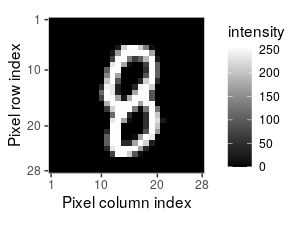
\includegraphics[width=0.4\textwidth]{figure-fashion-mnist-one-example}
  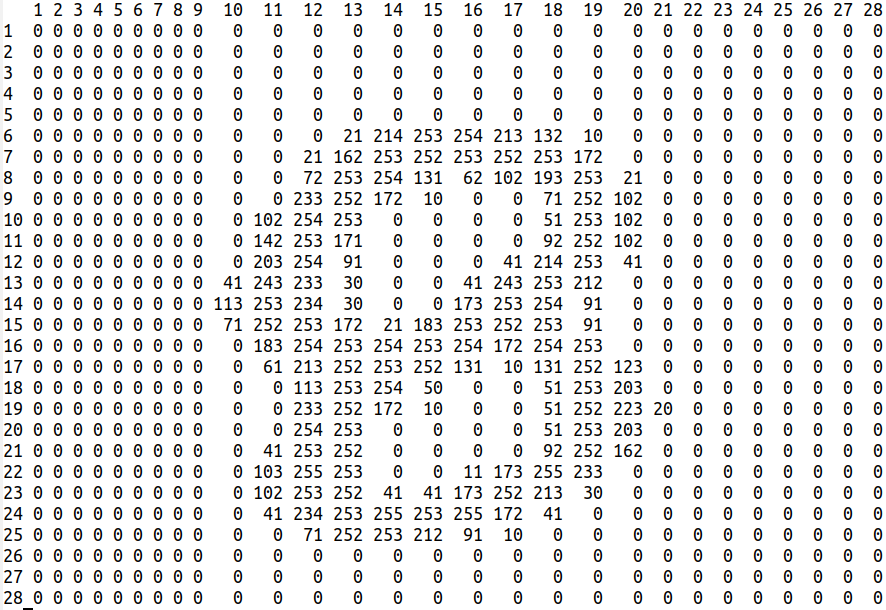
\includegraphics[width=0.4\textwidth]{screenshot-8-matrix-values}
  \caption{One example/observation with label 8 in the MNIST data
  set. \textbf{Left:} representation as greyscale
  image. \textbf{Right:} representation as $28 \times 28$ matrix;
  each of the 784 elements is an integer value from 0 to 255.}
  \label{fig:mnist-one-example}
\end{figure}

\begin{figure}
  \centering
  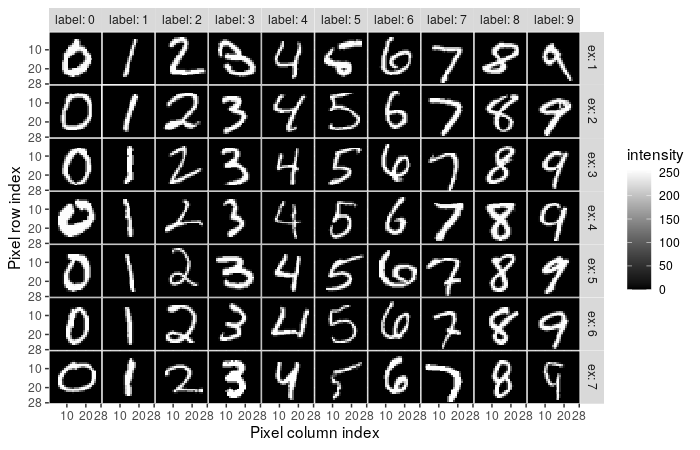
\includegraphics[width=0.49\textwidth]{figure-fashion-mnist-digits}
  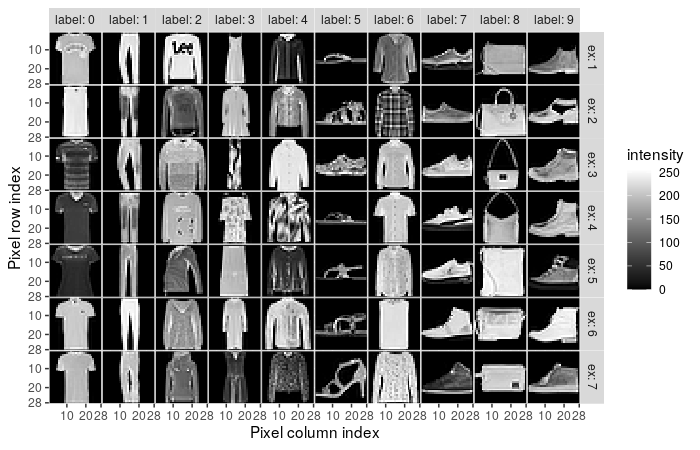
\includegraphics[width=0.49\textwidth]{figure-fashion-mnist-fashion}
  %   \\
  %   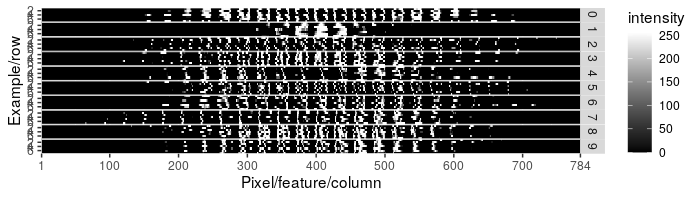
\includegraphics[width=0.49\textwidth]{figure-fashion-mnist-digits-design}
  %   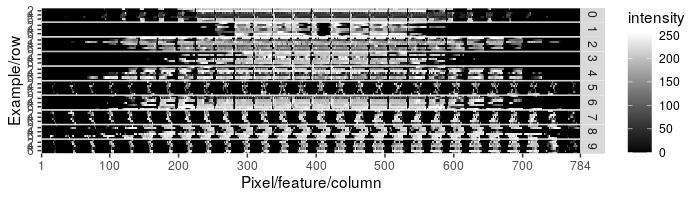
\includegraphics[width=0.49\textwidth]{figure-fashion-mnist-fashion-design} 
  \caption{Seven example images from each class/label in the original MNIST digits
  (left) and Fashion-MNIST (right) data sets. For each data set
  different label values from 0 to 9 appear are shown in panels
  from left to right, and different examples/observations are
  shown in panels from top to bottom.} 
  \label{fig:fashion-mnist}
\end{figure}

\end{document}
